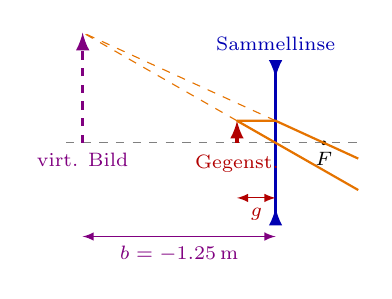
\begin{tikzpicture}[>=latex, scale=0.7, font=\scriptsize]
        \draw[gray, dashed] (-3.8,0) -- (1.6,0);
        % Sammellinse: Pfeile nach aussen
        \draw[blue!70!black, very thick, >-<] (0,-1.5) -- (0,1.5);
        \node[blue!70!black, above] at (0,1.5) {Sammellinse};
        % Gegenstand
        \draw[red!70!black, very thick, ->] (-0.7,0) -- (-0.7,0.4);
        \node[red!70!black, below=1pt] at (-0.7,0) {Gegenst.};
        % Brennpunkt
        \fill (0.875,0) circle (1.2pt) node[below] {$F$};
        % Strahl 1: parallel, danach durch F
        \draw[orange!90!black, thick] (-0.7,0.4) -- (0,0.4) -- (1.5,-0.286);
        \draw[orange!90!black, dashed] (0,0.4) -- (-3.5,2.0);
        % Strahl 2: durch die Linsenmitte
        \draw[orange!90!black, thick] (-0.7,0.4) -- (1.5,-0.857);
        \draw[orange!90!black, dashed] (-0.7,0.4) -- (-3.5,2.0);
        % virtuelles Bild
        \draw[violet, very thick, dashed, ->] (-3.5,0) -- (-3.5,2.0);
        \node[violet, below] at (-3.5,0) {virt. Bild};
        % Masse
        \draw[red!70!black, <->] (-0.7,-1.0) -- (0,-1.0) node[midway, below] {$g$};
        \draw[violet, <->] (-3.5,-1.7) -- (0,-1.7) node[midway, below] {$b=-1.25\,$m};
    \end{tikzpicture}